\documentclass[letterpaper, 12pt]{article}
\usepackage[english]{babel}
\usepackage{graphicx}
\usepackage{hyperref}
\usepackage{booktabs}

\begin{document}

\begin{titlepage}
\centering
	{\LARGE RoboJackets IGVC}\\
	\vspace{1cm}
	{\Large IGVC Motor and Light Control Board 2017}\\
	\vfill
	{\large Created at November 18, 2017}\\
	\vspace{1cm}
	{\large Last Edited at \today\par}
\end{titlepage}

\tableofcontents

\pagebreak

\section{Overview}
This document explained the function of the Motor and Light Control Board (referred as \emph{motor board} in the following) on \textbf{RoboJackets} IGVC subteam robot \textbf{Jessi} in year 2017 - 2018 and showed how the board is designed with regards to its need, capability and limitation. This document is created in the hope that future RJ members can have a good understanding of the robot without unnecessary effort. \vspace{6pt}\\
The motor board is the interface between Jessi's software control and her motor. IGVC software team completes path-planning on the two onboard Intel NUC computing units and will send command to the motor board. The motor board will then tune the value according to PID tuner and send it to the sabertooth motor controller, which will then power the motor.\\
\begin{figure}[h]
\centering
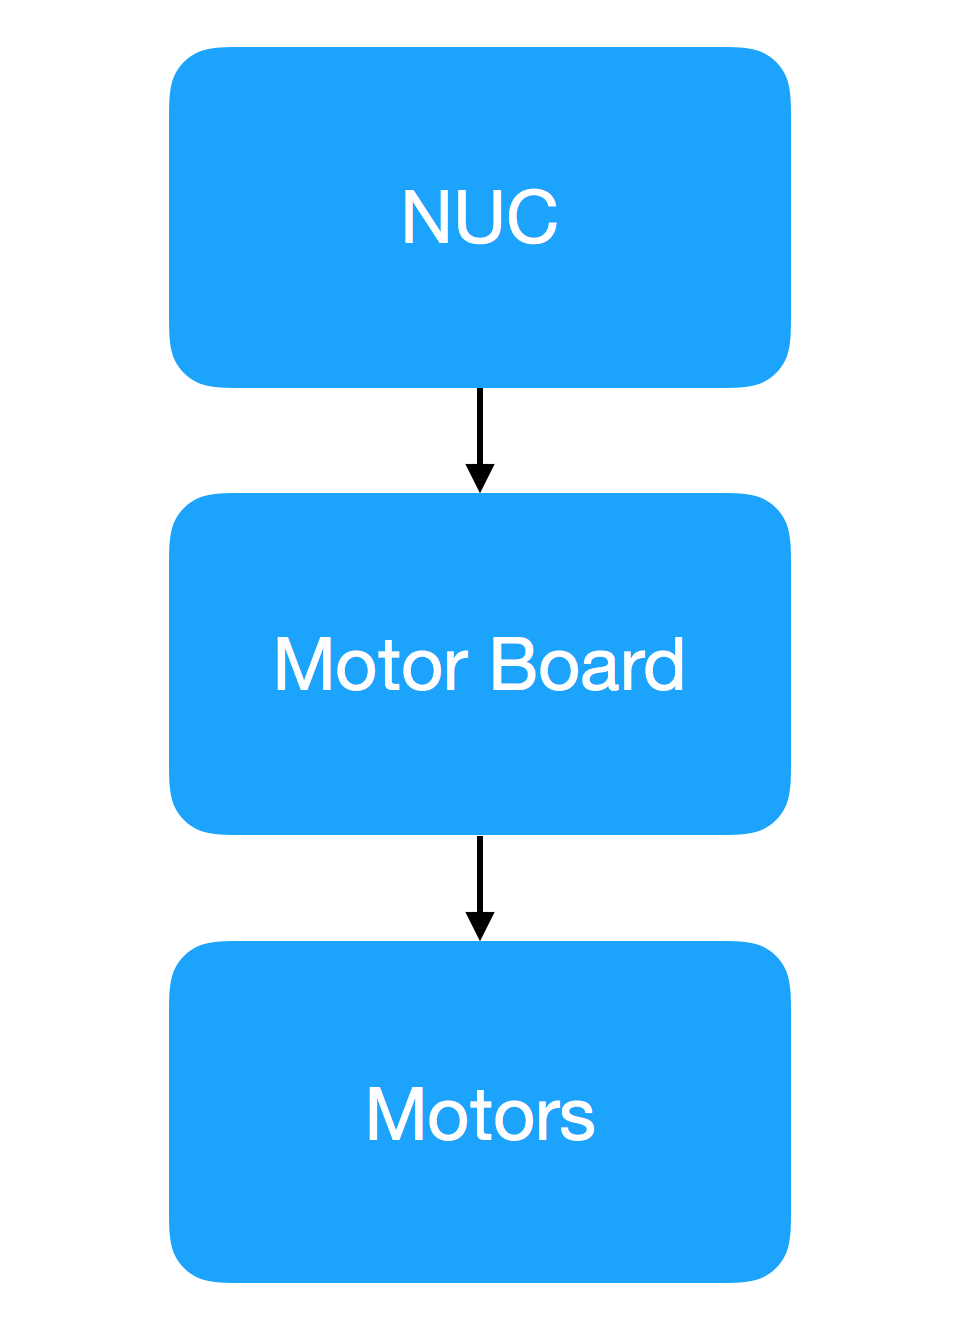
\includegraphics[width=0.5\textwidth]{UpandLow.png}
\caption{Motor Board's Data Input and Output}
\end{figure}

The primary function of the motor board is to ensure the DC motors are operating at the speed desired by the NUCs. Secondary functions include controlling the LED under-glow, monitoring battery voltage, E-stop status as well as Safety Light. The board also contained two ports for interfacing with OSMCs, a legacy motor controller module RJ used in the past. Each functioning circuits can operate independently from each other. \vspace{6pt}\\
The motor board is controlled by an mbed NXP LPC1768 microcontroller. More details here: \url{https://os.mbed.com/platforms/mbed-LPC1768/} \vspace{6pt}\\


\section{Hardware}
\subsection{Controlling Unit}
\subsection{Motor Control Circuit}
Subsection of motor control circuit 
\pagebreak
\subsection{Light Control Circuit}
Subsection of light control circuit
\pagebreak
\subsection{Power System}
Four voltage level runs through this board. 

\begin{table}[h]
\caption{Summary of functions of Voltage Levels}
\centering
\begin{tabular}{p{2cm}p{2cm}}
\toprule
\midrule
asdasd\\
\bottomrule
\end{tabular}
\end{table}

\pagebreak
\subsection{Board Layout}
Explanation of how the board is laid out, details including components not covered in schematics. 
\pagebreak

\section{Firmware}
\subsection{Controlling the board}
\pagebreak
\subsection{Interacting with Peripheral Devices}
\pagebreak

\section{Miscellaneous}
\subsection{Legacy Interfaces}
\pagebreak
\subsection{Expected Future Usage}
\pagebreak

\section{Special Regards}
\pagebreak
\end{document}